% ==============================================================================
%
%                                    DVG303
%                  Objektorienterad design och programmering
%                                Laboration #1
%
% Author:   Jonas Sjöberg
%           Högskolan i Gävle
%           tel12jsg@student.hig.se
%           https://github.com/jonasjberg
%
% License:  Creative Commons Attribution-NonCommercial-ShareAlike 4.0
%           International.  See LICENSE.md for full licensing information.
% ==============================================================================

\documentclass[11pt,a4paper]{article}
\usepackage[utf8]{inputenc}
\inputencoding{utf8}
\usepackage[swedish]{babel}
\usepackage[swedish]{isodate}
\usepackage[T1]{fontenc}
\usepackage{lmodern}
\usepackage{fullpage}

\usepackage{textcomp}
\usepackage{url}
\usepackage{graphicx}

\usepackage{minted}
\usemintedstyle{bw}

\usepackage{verbatim}
\usepackage{fancyvrb}
\usepackage{listings}

\usepackage[pdfusetitle,bookmarks=true,
 bookmarksnumbered=true,bookmarksopen=false,
 breaklinks=false,pdfborder={0 0 0},backref=false,
 colorlinks=false]{hyperref}

\newmintedfile[javacode]{java}{
%bgcolor=mintedbackground,
%fontfamily=tt,
fontsize=\footnotesize,
linenos=true,
numberblanklines=true,
numbersep=12pt,
numbersep=5pt,
frame=lines,
framesep=2mm,
funcnamehighlighting=true,
tabsize=4,
obeytabs=false,
mathescape=false
samepage=false,
showspaces=false,
showtabs =false,
texcl=false,
}

\renewcommand{\thesubsection}{\thesection(\alph{subsection})}
%\renewcommand{\thesubsection}{(\alph{subsection})}

\title{DVG303 \\ Objektorienterad design och programmering \\ Laboration 1}

\author{\\
  Jonas Sjöberg\\
  860224\\
  Högskolan i Gävle\\
  \texttt{tel12jsg@tudent.hig.se}\\
  \texttt{https://github.com/jonasjberg}\\
}


\date{}

\begin{document}
    \maketitle

    \begin{center}
    \begin{tabular}{l r}
        Datum: & \isodate \today \par \\
        Kursansvarig lärare: & 
    \end{tabular}
    \end{center}

    \medskip

    \begin{abstract}
        Laborationsrapport för
        \emph{DVG303 -- Objektorienterad design och programmering},
        Högskolan i Gävle, Höstterminen 2015.
    \end{abstract}

    \newpage
    \setcounter{tocdepth}{3}
    \tableofcontents
    \listoffigures
    \newpage

    %% ==============================================================================
%
%                                    DVG303
%                  Objektorienterad design och programmering
%                                Laboration #1
%
% Author:   Jonas Sjöberg
%           Högskolan i Gävle
%           tel12jsg@student.hig.se
%           https://github.com/jonasjberg
%
% License:  Creative Commons Attribution-NonCommercial-ShareAlike 4.0
%           International.  See LICENSE.md for full licensing information.
% ==============================================================================

\section{Introduktion}\label{sec:intro}

\subsection{}\label{sec:uppg1a}
\subsubsection*{Övergripande beskrivning}
Det här är den första av tre laborationer i objektorienterad design och
programmering. Under laborationerna kommer programvara att utvecklas från en
specifikation. 
% TODO: Syfte (modern mjukvaruutveckling, revisionskontroll, dokumentation ..)

\subsubsection*{Specifikation}
Efterfrågad funktionalitet för programmet beskrivs enligt UML-standard i 
Figur~\ref{fig:usecase}.

\begin{figure}[htbp]
\centering
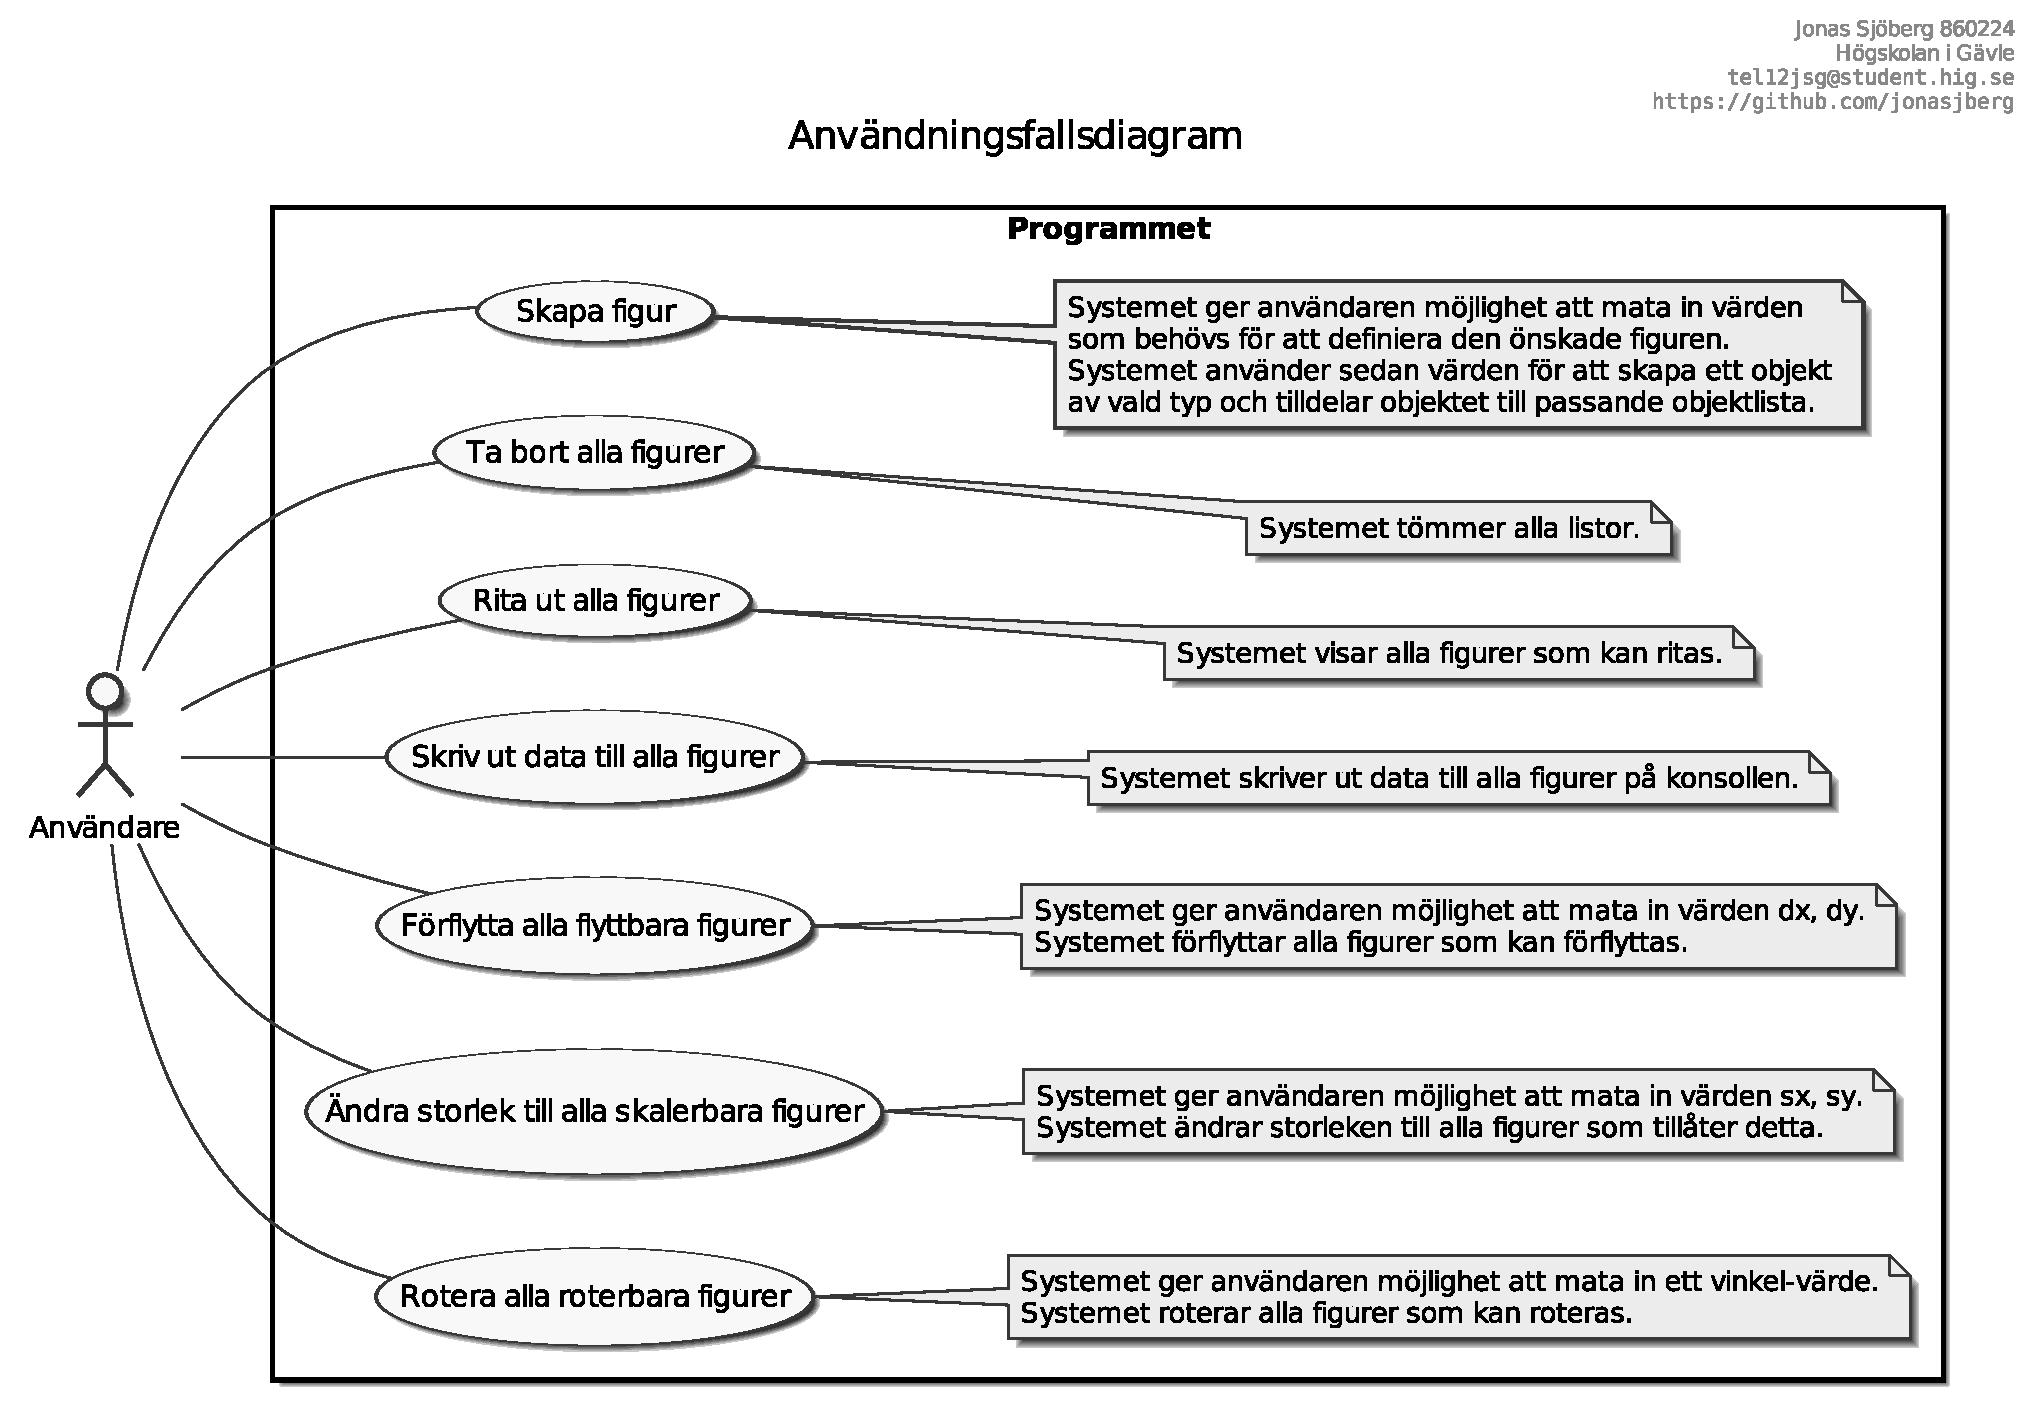
\includegraphics[width=\linewidth]{diagram/usecase.eps}
\caption{Användningsfallsdiagram \emph{("use case diagram")}}
\label{fig:usecase}
\end{figure}




    % ==============================================================================
%                                    DVG303
%                  Objektorienterad Design och Programmering
%                                Laboration #1
%
% Author:   Jonas Sjöberg
%           Högskolan i Gävle
%           tel12jsg@student.hig.se
%           https://github.com/jonasjberg
%
% License:  Creative Commons Attribution-NonCommercial-ShareAlike 4.0
%           International.  See LICENSE.md for full licensing information.
% ==============================================================================

\renewcommand{\thesubsection}{(\alph{subsection})}

\section{Uppgift 1}\label{sec:uppg1}
% \addcontentsline{toc}{section}{Uppgift 1}


\subsection{}\label{sec:uppg1a}
\subsubsection*{Frågeställning}
Modellera klasserna som representerar konkreta geometriska figurer som ska
kunna hanteras i programmet och därför ska ingå i programmets datamodell:
Punkt, linje, triangel, cirkel, rektangel.
\par Beskriv klasserna på ett liknande sätt som i kursboken, kap 2.2, på sida
65 - tredje upplaga.  Skapa dessutom ett UML-klassdiagram för modellen.
\par Motivera era beslut: Varför skapade ni modellen som den är? Varför har
klasserna de attribut och operationer så som ni valde?

\subsubsection*{Lösning}
Figurerna beskrivs av ett visst antal punkter eller positioner som
representeras av \texttt{Vertex2D}-instanser. Alla figurer består av minst ett
\texttt{Vertex2D}-objekt som representerar figurens mittpunkt. Figurerna kan
delas upp i två separata grenar i arvshierarkin, \texttt{Figure} och
\texttt{SimpleFigure}.  Skillnaden mellan Figure och SimpleFigure är hur många
punkter de lagrar för att beskriva figuren de representerar.  Figurer som kan
beskrivas med bara en \texttt{Vertex2D}-instans, figurens position, ärver från
\texttt{SimpleFigure}; punkt, cirkel och ellips.  Figurer som består av fler
\texttt{Vertex2D}-objekt, ärver från \texttt{Figure}.  Klassen \texttt{Figure}
lagrar sina punkter i en lista för enkel åtkomst.  Det möjliggör också
skapandet av figurer med ett godtyckligt antal punkter.

\begin{figure}[htbp]
\centering
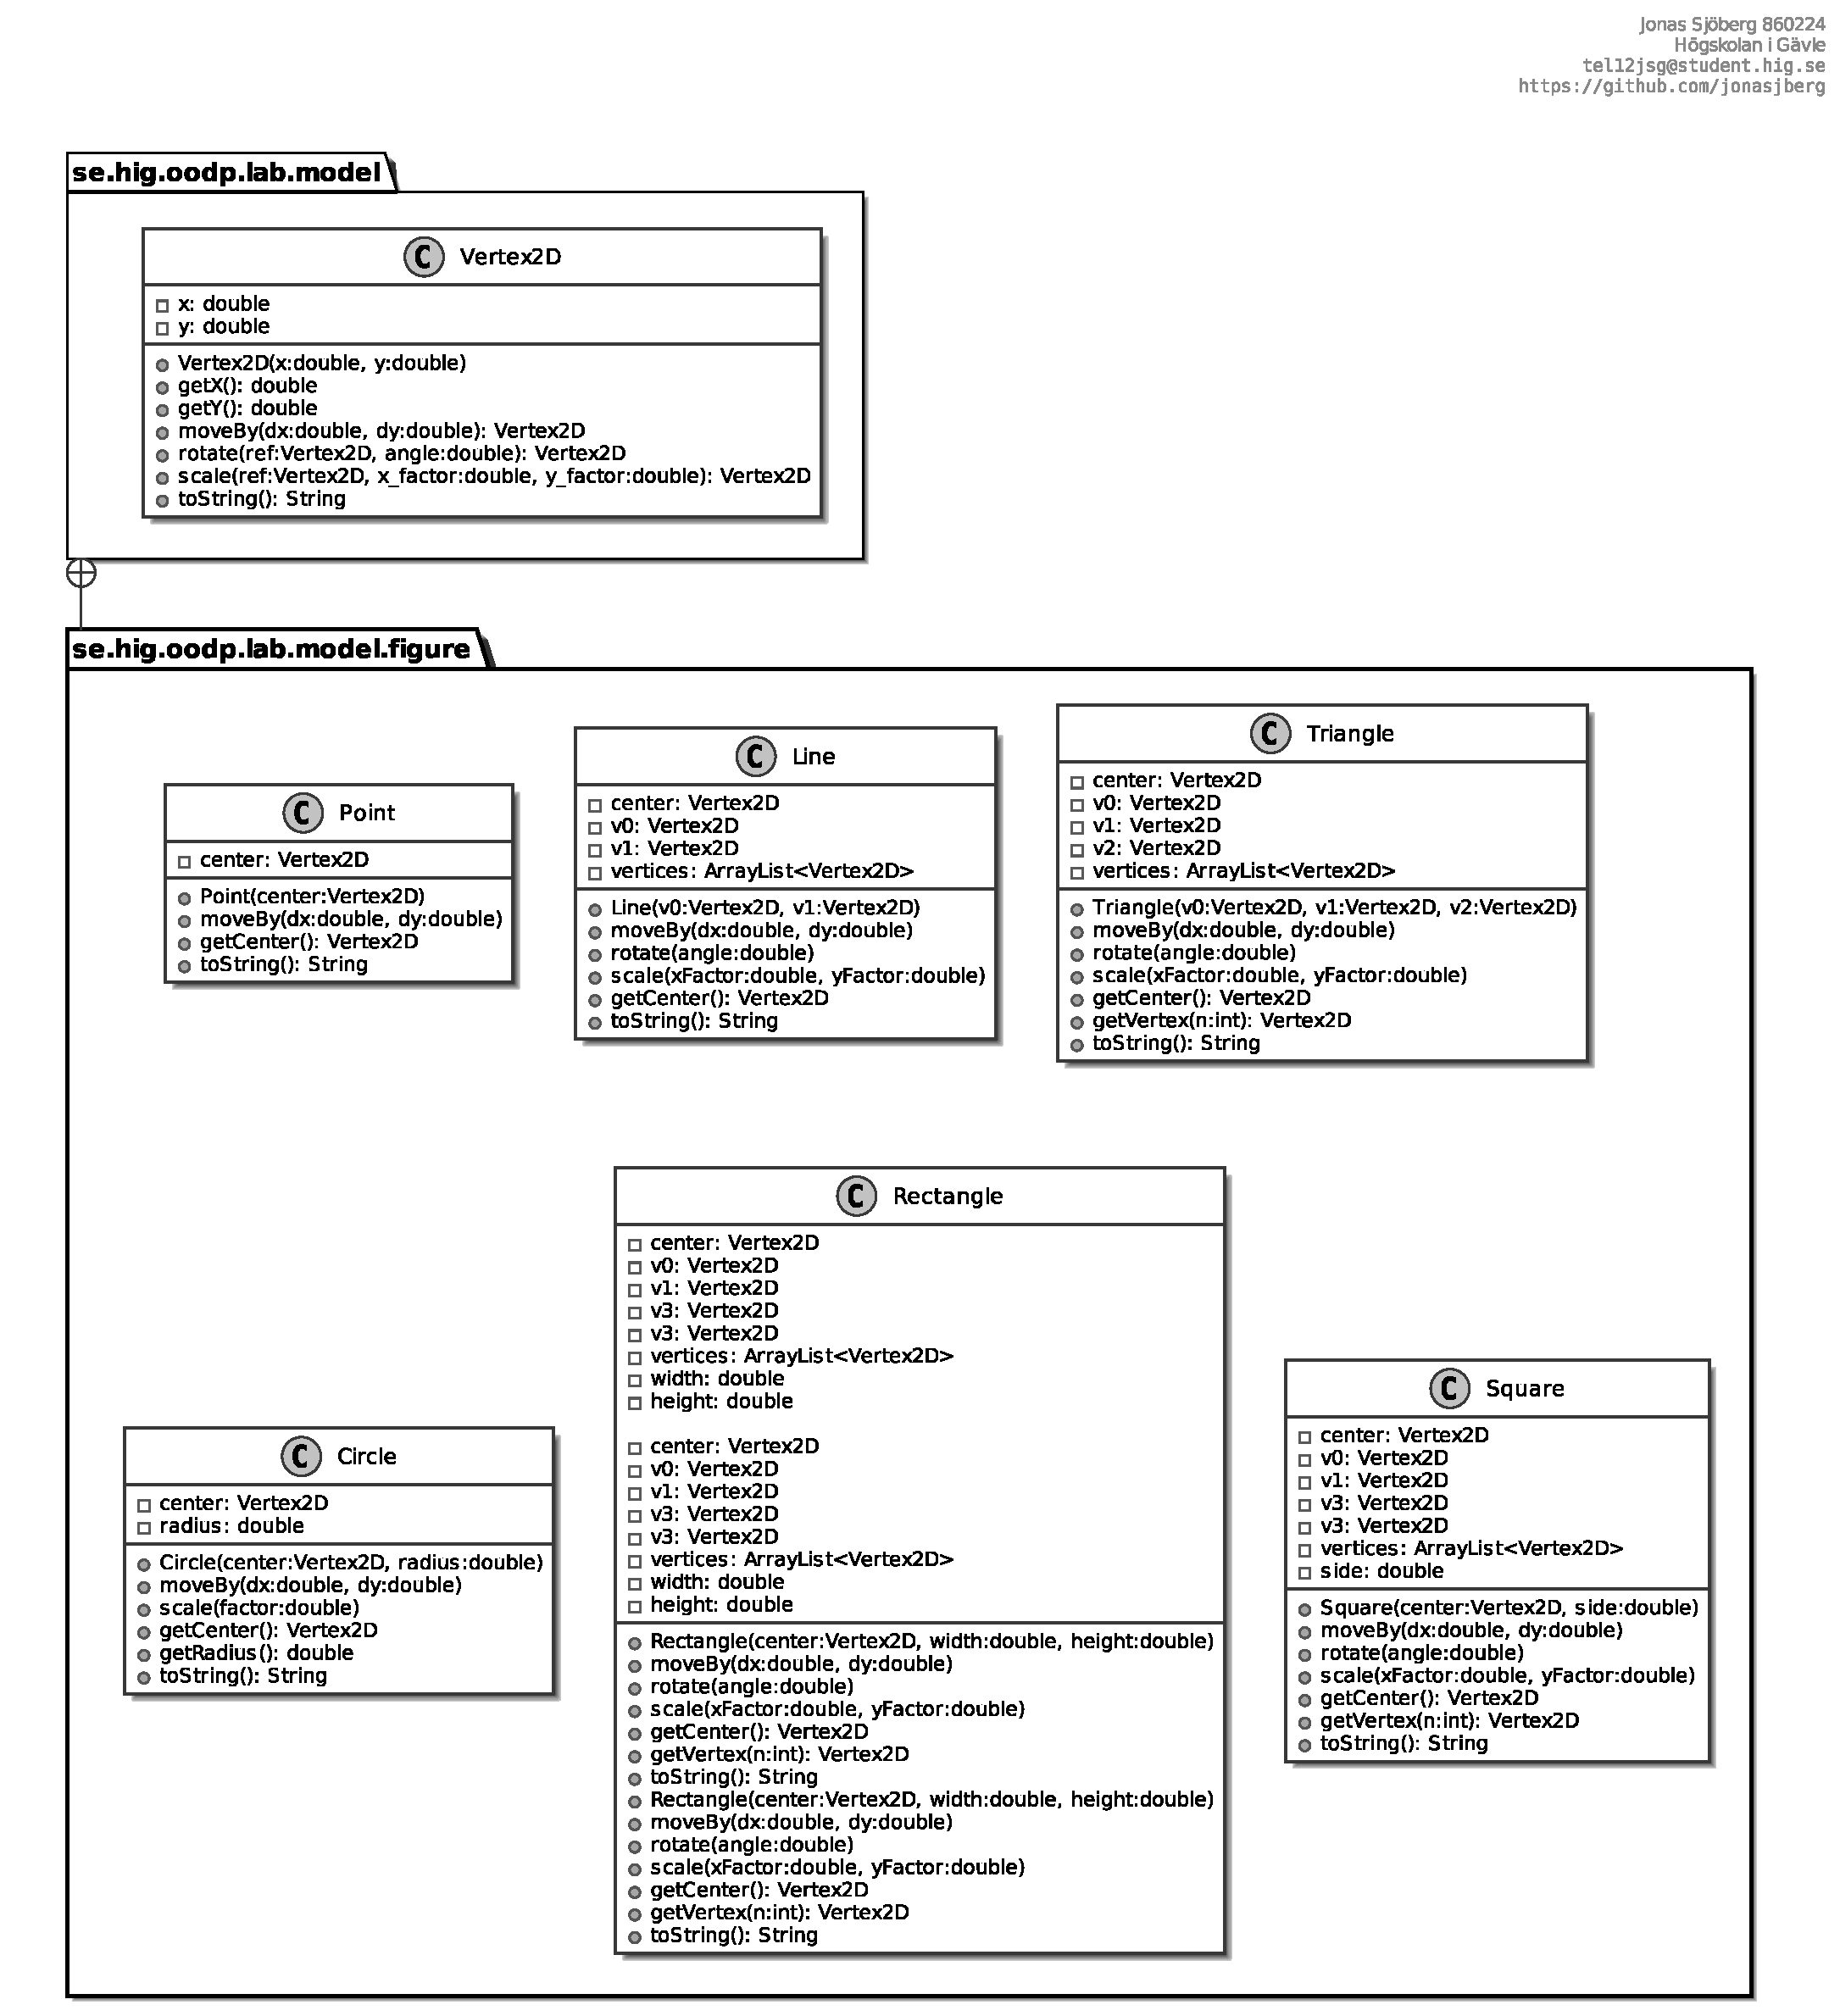
\includegraphics[width=\linewidth]{diagram/uppgift1.eps}
\caption{Uppgift~1\ref{sec:uppg1a}: UML-diagram för geometriska figurer
(\texttt{diagram/uppgift1.eps})}
\label{fig:uppg1a}
\end{figure}

\par UML-klassdiagrammet återfinns i Figur~\ref{fig:uppg1a}, samt bifogad fil.


\subsection{}\label{sec:uppg1b}
\subsubsection*{Frågeställning}
Implementera klasserna som ingår i klassdiagrammet och skapa JUnit-tests för
att testa koden!

\subsubsection*{Lösning}
Se bifogad källkod, klasserna finns i paketen
\texttt{se.hig.oodp.lab.model.simplefigure} \\ och
\texttt{se.hig.oodp.lab.model.figure}.



\subsection{}\label{sec:uppg1c}
\subsubsection*{Frågeställning}
Vilken relation ser ni mellan klassen Vertex2D och figurklasserna resp. mellan
instanser av Vertex2D och instanser av figurklasserna? På vilket sätt
återspeglas relationen i klassdiagrammet? Ge en förklaring!

\subsubsection*{Lösning}
Klassen \texttt{Vertex2D} är en del av figurklasserna. Figurklasserna består
av minst en \texttt{Vertex2D} som utgör figurens mittpunkt. Figurklasserna
har en varsin lista där ett godtyckligt antal \texttt{Vertex2D}-objekt kan
lagras, antalet beror på vilken figur subklassen representerar.

    %% ==============================================================================
%
%                                    DVG303
%                  Objektorienterad design och programmering
%                                Laboration #1
%
% Author:   Jonas Sjöberg
%           Högskolan i Gävle
%           tel12jsg@student.hig.se
%           https://github.com/jonasjberg
%
% License:  Creative Commons Attribution-NonCommercial-ShareAlike 4.0
%           International.  See LICENSE.md for full licensing information.
% ==============================================================================

\section{Uppgift 2}\label{sec:uppg2}

\subsection{}\label{sec:uppg2a}
\subsubsection*{Frågeställning}
En superklass kan innehålla attribut och operationer som är gemensamma
för ett antal klasser.  Beskriv en superklass till klasserna ni skapade i 
uppgift 1! Beskrivningen ska innehålla information om vilka attribut det ska 
finnas i superklassen och vilka meddelanden (kommandon och frågor) man kan 
skicka till instanser av superklasstypen.  Förklara varför ni bestämde er 
för just den uppsättning attribut/operationer som ni valde!


\subsubsection*{Lösning}
Figurerna beskrivs av ett visst antal punkter eller positioner som representeras
av \texttt{Vertex2D}-instanser. Alla figurer består av minst ett
\texttt{Vertex2D}-objekt som representerar figurens mittpunkt. Figurerna kan
delas upp i två separata grenar i arvshierarkin, \texttt{Figure} och
\texttt{SimpleFigure}.  Skillnaden mellan Figure och SimpleFigure är hur många
punkter de lagrar för att beskriva figuren de representerar.  Figurer som kan
beskrivas med bara en \texttt{Vertex2D}-instans, figurens position, ärver från
\texttt{SimpleFigure}; punkt, cirkel och ellips.  Figurer som består av fler
\texttt{Vertex2D}-objekt, ärver från \texttt{Figure}.  Klassen \texttt{Figure}
lagrar sina punkter i en lista för enkel åtkomst.  Det möjliggör också
skapandet av figurer med ett godtyckligt antal punkter.


\subsection{}\label{sec:uppg2b}
\subsubsection*{Frågeställning}
Ska superklassen vara en abstrakt klass eller inte? Diskutera vad som talar
emot och vad som talar för!

\subsubsection*{Lösning}
Klasserna \texttt{SimpleFigure} och \texttt{Figure} är både abstrakta av den
anledningen att vi sannolikt inte kommer att behöva instantiera någon odefinerad
figur. Möjligheten att skapa t.ex. en polygon med ett godtyckligt antal punkter
från figurklasserna talar emot att de är abstrakta, det skulle vara möjligt att
skapa odefinerade figur-objekt och efter att de skapats namnge dem till 
rätt figur (punkt, kvadrat, triangel, etc..) efter det antal punkter figuren 
instantierats med och dessa punkters position.
I det här fallet valde jag ändå att göra figurklasserna abstrakta och låta
subklasserna punkt, kvadrat, triangel, etc.. ärva från superklasserna och
utgöra faktiska, instantierbara objekt.
De olika figurerna har fält och metoder som gör dem unika, en cirkel har t.ex.
en radie medan en ellips har en bredd och höjd.


\subsection{}\label{sec:uppg2c}
\subsubsection*{Frågeställning}
Uppdatera klassdiagrammet från uppgift 1, så att den nya klassen ingår i
modellen samt relationerna mellan superklassen och befintliga klasser!

\subsubsection*{Lösning}
\par UML-klassdiagrammet och arvshierarkin återfinns i Figur~\ref{fig:uppg2a},
 samt bifogad fil .

%\begin{figure}[htbp]
\begin{sidewaysfigure}[ht]
\centering
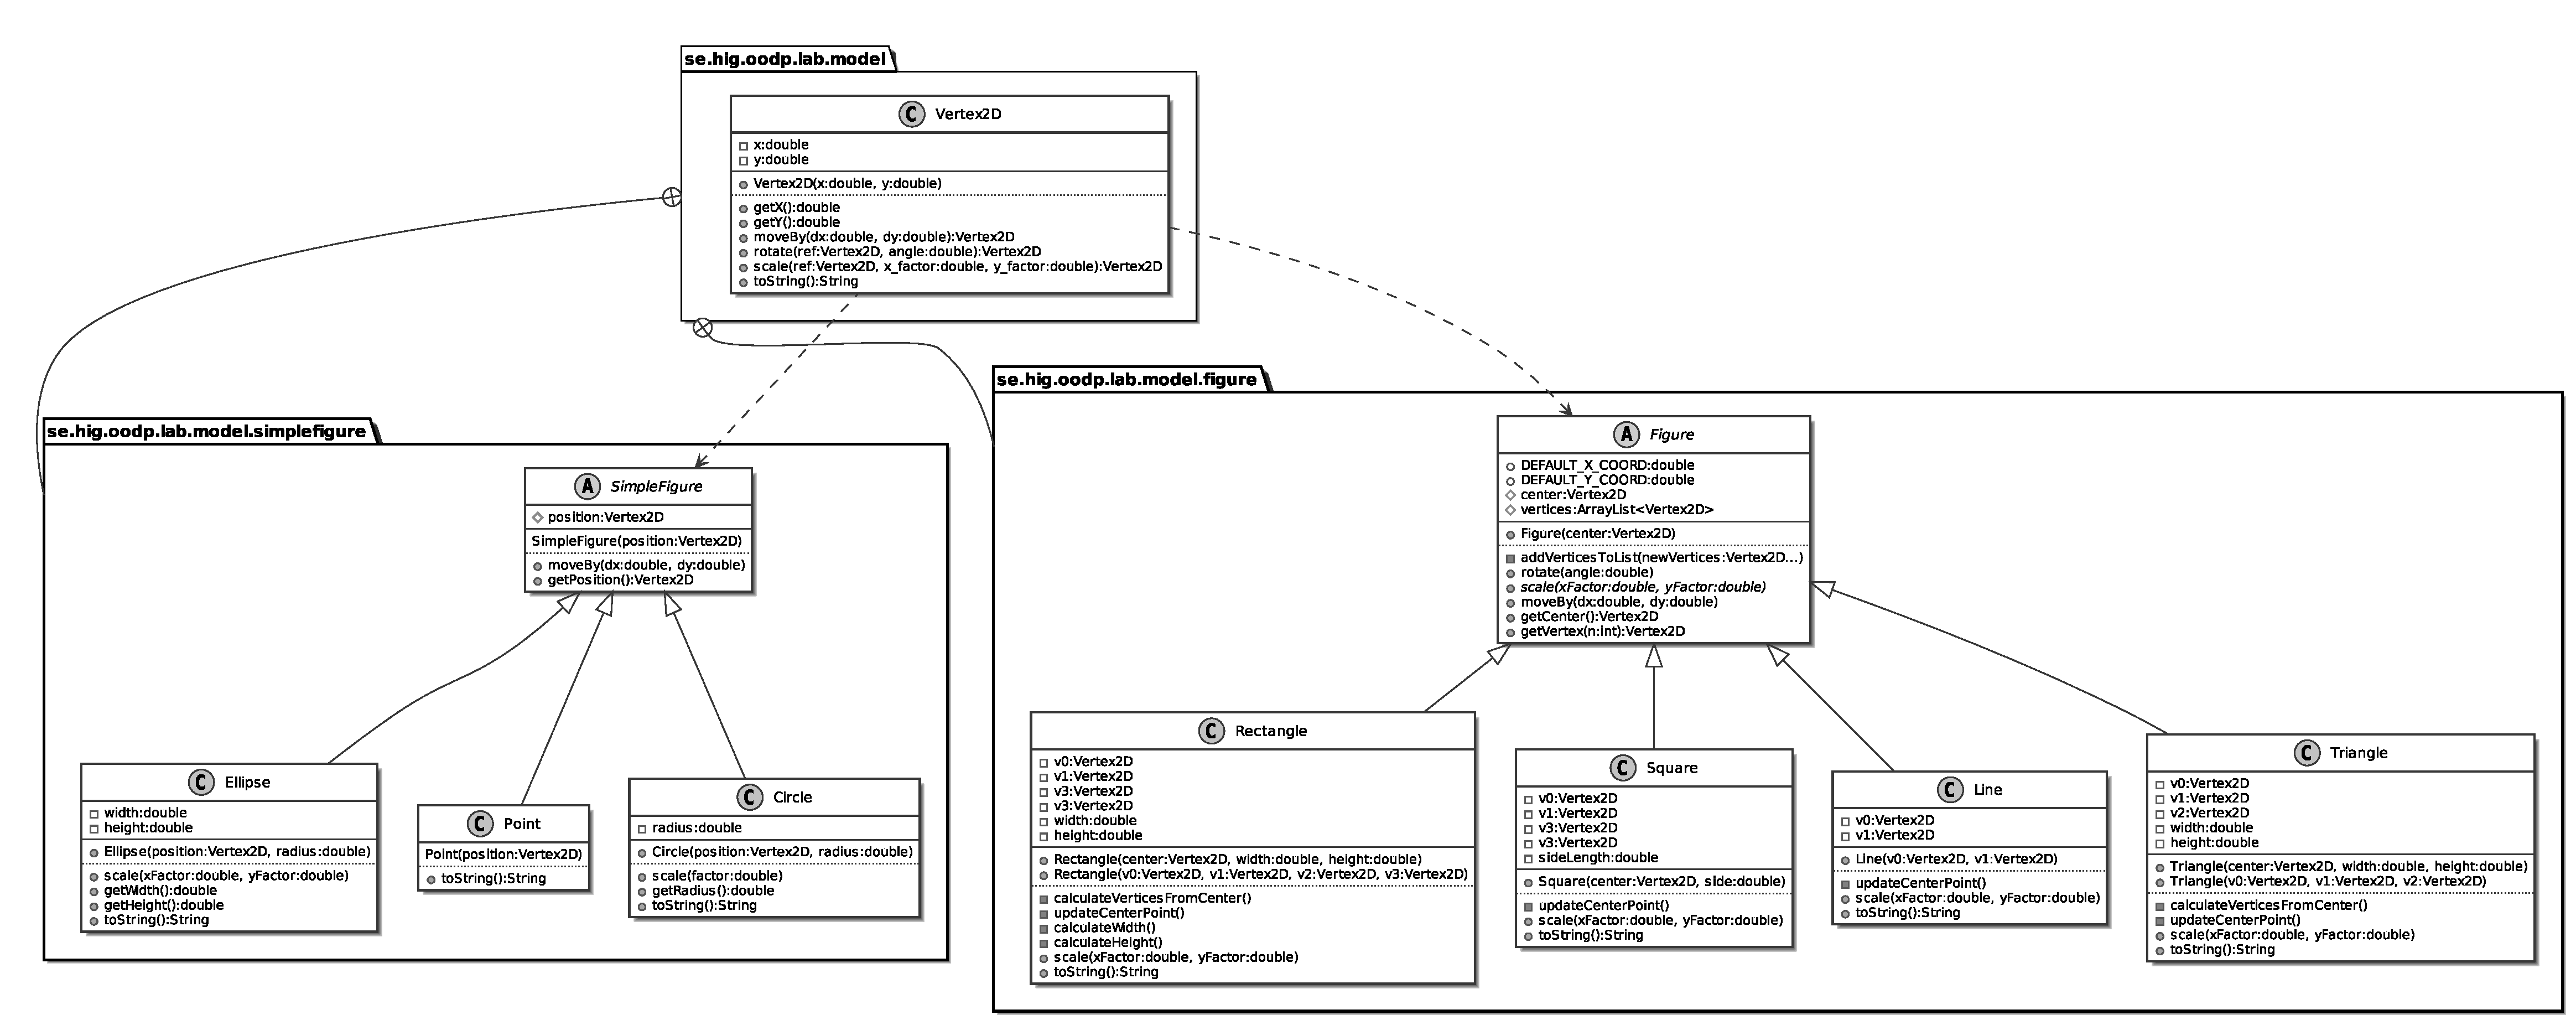
\includegraphics[width=\linewidth]{diagram/uppgift2.eps}
\caption{Uppgift~2\ref{sec:uppg2c}: UML-diagram för geometriska figurer
(\texttt{diagram/uppgift2.eps})}
\label{fig:uppg2a}
\end{sidewaysfigure}


\subsection{}\label{sec:uppg2d}
\subsubsection*{Frågeställning}
Implementera modellen som ni skapade i (c), dvs. aktualisera koden från
uppgift 1 så att den motsvarar klassdiagrammet från (c)!
Använd testen som ni utvecklade i uppgift 1 för att visa att klasserna fungerar
som förut!

\subsubsection*{Lösning}
Se bifoad kod.

    %% ==============================================================================
%
%                                    DVG303
%                  Objektorienterad design och programmering
%                                Laboration #1
%
% Author:   Jonas Sjöberg
%           Högskolan i Gävle
%           tel12jsg@student.hig.se
%           https://github.com/jonasjberg
%
% License:  Creative Commons Attribution-NonCommercial-ShareAlike 4.0
%           International.  See LICENSE.md for full licensing information.
% ==============================================================================

\renewcommand{\thesubsection}{(\alph{subsection})}

\section{Uppgift 3}\label{sec:uppg3}

\subsection{}\label{sec:uppg3a}
\subsubsection*{Frågeställning}
Betrakta nu modellen en gång till: Ser ni likheter när det gäller objektens
beteenden? Vilka är dessa? Ge en Beskrivning!

\subsubsection*{Lösning}
Alla figurer behöver någon mekanism för att flytta på sig och det kan tänkas
att alla figurer skulle kunna använda sig av sammma logik för att utföra
förflyttningen. Exempel på hur det skulle kunna implementeras är med en
\texttt{move()}-metod i en gemensam superklass som itererar genom en lista av
\texttt{Vertex2D}-punkter och flyttar varje punkt för sig. Alla figurer kan
uttryckas med en lista av punkter och kan således ärva från en gemensam
superklass.
\par Ett annat exempel är rotering, som inte är applicerbart för vissa figurer,
t.ex. cirkeln. Det kan vara konceptuellt möjligt att rotera en perfekt cirkel,
men i det här fallet så skulle cirkelns interna läge inte förändras, och
den grafiska representationen skulle inte heller komma att ändras.
Alternativet till ett interface \texttt{Rotatable} i fallet med cirkeln är att
\texttt{rotate()}-metoden i cirkel-klassen blir ersatt med en tom metod genom 
\emph{override}.


\subsection{}\label{sec:uppg3b}
\subsubsection*{Frågeställning}
Utöka nu klassdiagrammet en gång till: Lägg till minst ett interface som
deklarerar någon metod som passar till det som ni beskrev ovan. Låt klasserna
implementera interfacet ifall det passar!

\subsubsection*{Lösning}
Jag bestämde mig för att lägga till interfacen \texttt{Movable},
\texttt{Rotatable} och \texttt{Scalable}. Detta med motiveringen att det
är operationer som efterfrågas i användningsfallsdiagrammet och som de olika
figurerna kan komma att behöva utföra på olika vis, beroende på figur. 
Avvägning gjordes mot att göra en enklare design som förlitar sig mer på arv
och \emph{override} av superklassers metoder. Det uppdaterade klassdiagrammet
återfinns i Figur~\ref{fig:uppg3b}.

%\begin{figure}[htbp]
\begin{sidewaysfigure}[ht]
\centering
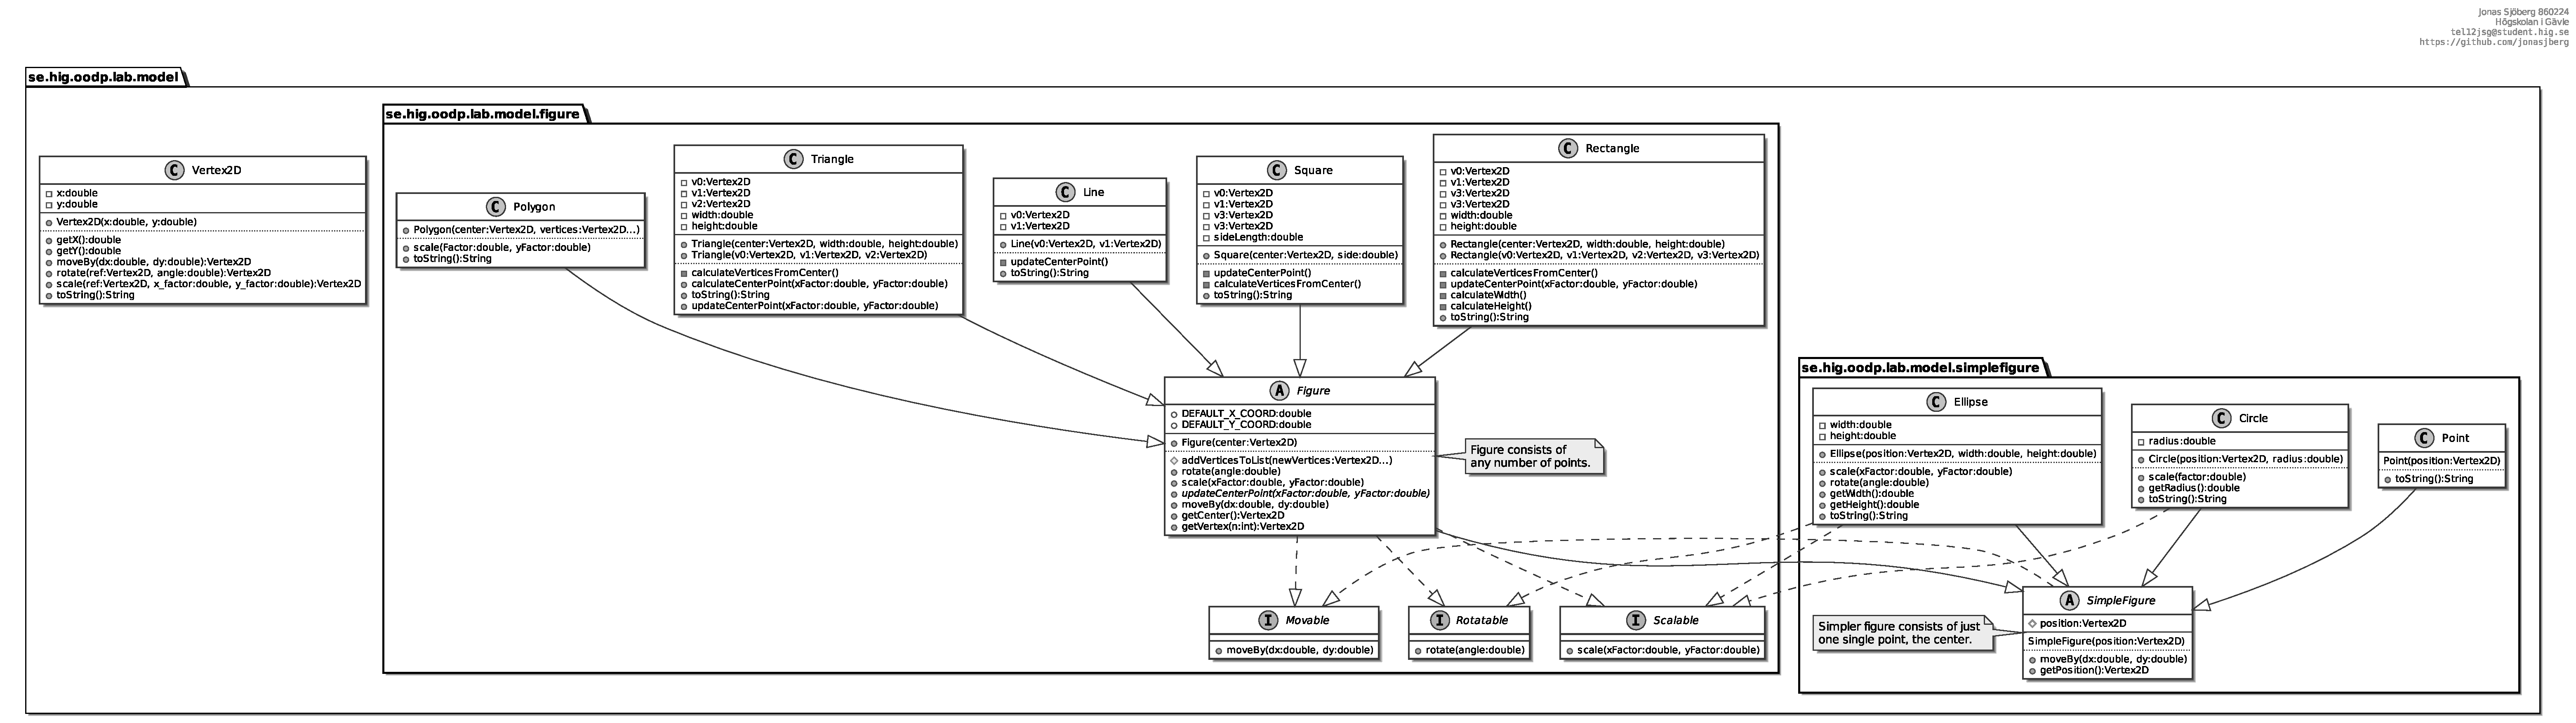
\includegraphics[width=\linewidth]{diagram/uppgift3.eps}
\caption{Uppgift~3\ref{sec:uppg2c}: UML-diagram för geometriska figurer
(\texttt{diagram/uppgift3.eps})}
\label{fig:uppg3b}
\end{sidewaysfigure}



\subsection{}\label{sec:uppg3c}
\subsubsection*{Frågeställning}
Uppdatera koden från uppgift 2 så att det motsvarar den utökade modellen från
(b)!

\subsubsection*{Lösning}
Se bifogad kod för implementering.




\end{document}

